\subsection{Ontology}

\begin{frame}
	An ontology is an explicit, \alert{formal knowledge representation} that express knowledge about a domain of application. This includes:
	\begin{itemize}
		\item Types of entities that exist in the domain\\
			\begin{itemize}
				\item e.g.: Person, Enterprise, $\ldots$
			\end{itemize}
		\item Properties of those entities\\
			\begin{itemize}
				\item e.g.: firstName, lastName, $\ldots$
			\end{itemize}
		\item Relationships among entities\\
			\begin{itemize}
				\item e.g.: motherOf, ownerOf, $\ldots$
			\end{itemize}
		\item Processes and events that happen with those entities\\
			\begin{itemize}
				\item e.g.: choosing best proposal, $\ldots$
			\end{itemize}
	\end{itemize}
\end{frame}

\begin{frame}
	\centering{\LARGE{How to represent ontologies?}}
	\pause
	\begin{block}{Web Ontology Language (OWL)}
		\begin{itemize}
			\item Created at 2004
			\item Developed by the W3C
			\item As a language to represent ontologies for the Semantic Web
		\end{itemize}
	\end{block}
\end{frame}

\begin{frame}
	\begin{figure}
		\centering
		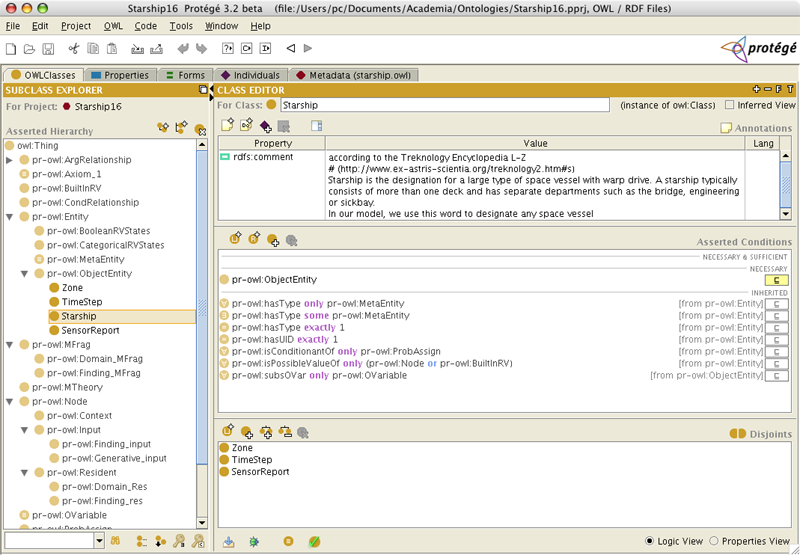
\includegraphics[width=\textwidth]{images/ontology_example}
		\caption{Protegé program}
	\end{figure}
\end{frame}